\section{Introduction and Related Work}
\frame{\sectionpage}


\begin{frame}[fragile]{SQL: Introduction}
    Given a SQL query, how is it executed?
    \begin{lstlisting}[language=SQL, caption= SQL query to execute.]
        SELECT MovieTitle
        FROM StarsIn
        WHERE StarName IN(
            SELECT name
            FROM MovieStar
            WHERE birthdate LIKE '%1960'
        );
    \end{lstlisting}
\end{frame}

\begin{frame}{SQL: Pipeline}
    \begin{figure}
        \centering
        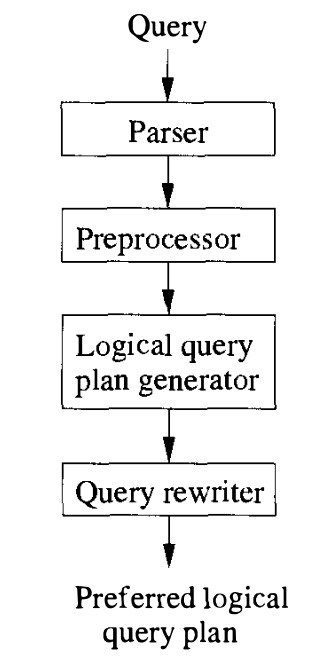
\includegraphics[scale=0.25]{query_processor.png}\\
        \caption{The pipeline for query processing}
        \label{fig:query_processor}
    \end{figure}
\end{frame}

\begin{frame}{SQL: Parser}
    \begin{figure}
        \centering
        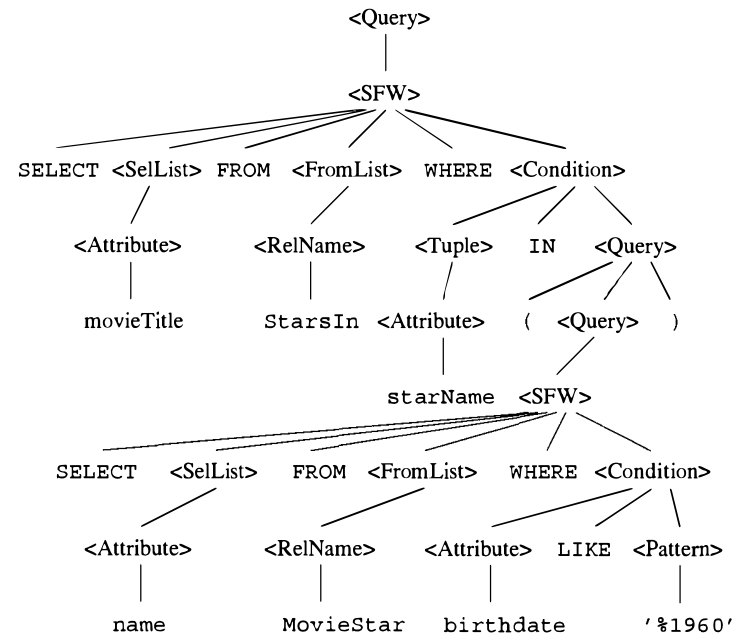
\includegraphics[scale=0.25]{parse_tree.png}\\
        \caption{An example of parse tree}
        \label{fig:prase_tree}
    \end{figure}
\end{frame}

\begin{frame}{SQL: Rewrite}
    Need to convert the query plan using Relational Algebra into a query plan which requires has lowest cost according to estimates.
\end{frame}

\begin{frame}[fragile]{SQL: Relational Algebra}
    \begin{figure}
        \centering
        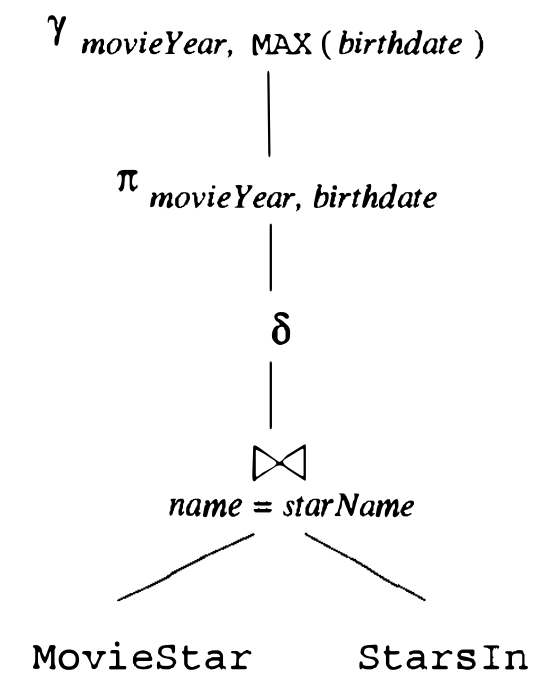
\includegraphics[scale=0.21]{join_pushdown1.png}
        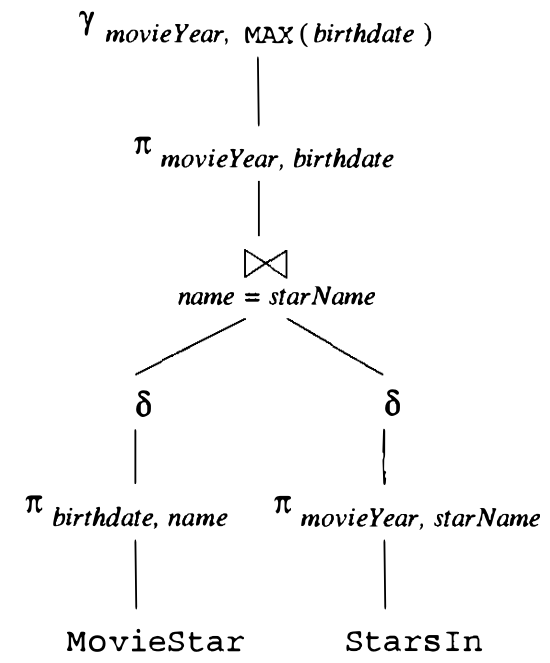
\includegraphics[scale=0.21]{join_pushdown2.png}
        \label{fig:j_1}
    \end{figure}
    \begin{lstlisting}[language=SQL]
    SELECT movieYear, MAX(birthdate) 
    FROM MovieStar, StarIn
    WHERE name=starName 
    GROUP BY movieYear;
    \end{lstlisting}
\end{frame}

\begin{frame}{SQL: Cost Estimation}
    \begin{enumerate}
        \item Give accurate estimates. No matter what method is used for executing query plans.
        \item Are easy to compute.
        \item Are logically consistent.
    \end{enumerate}
\end{frame}

\begin{frame}{SQL: Cost Calculation Methods}
    \begin{enumerate}
        \item Histogram
        \item Heuristics
        \item Top-Down
        \item Bottom-up
        \item Dynamic Programming
        \item Branch-and-Bound
        \item Hill Climbing
        \item Selinger-Style Optimization
    \end{enumerate}
\end{frame}

\begin{frame}[fragile]{SQL: Branch and Bound}
    \begin{lstlisting}[language=python]
    cost_upper_limit= +inf
    plan=[]
    while(can explore):
        if node has unexplored neighbours:
            explore node neighbour
            calculate cost of current plan
            if cost of plan >=cost_upper_limit:
                backtrack
            else:
                update plan
            if(complete plan and cost of plan < cost_upper_limit):
                optimal_plan=current_plan
                cost_upper_limit = cost of plan
        else:
            mark node as explored completely
            backtrack
    return optimal_plan
    \end{lstlisting}
\end{frame}

\begin{frame}{SQL: Physical Plan}
    \begin{enumerate}
        \item Algorithm selection(e.g. index scan, table scan, join method)
        \item Materialized or pipelined
        \item How relations are accessed
    \end{enumerate}
\end{frame}

\begin{frame}{Data Stream Processing}
    Modifying queries by changing graph topology and/ or operators to get better performance, as measured by
    \begin{enumerate}
        \item Throughput
        \item Latency
        \item Resource Usage.
    \end{enumerate}
    While preserving semantice of the original query.
\end{frame}

\begin{frame}{Stream Graph}
    \begin{figure}
        \centering
        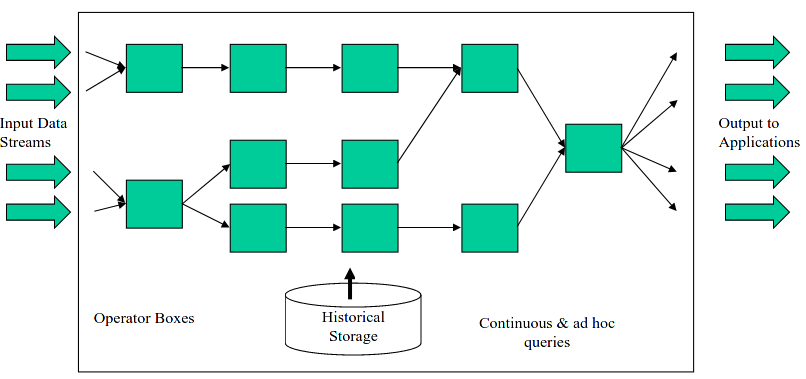
\includegraphics[scale=0.5]{dsms_dag.png}
        \label{fig:j_1}
    \end{figure}
\end{frame}

\begin{frame}{Possible Optimization for Stream Query Processing}
    \begin{itemize}
        \item Batching
        \item Placement
        \item State sharing
        \item Load Balancing
        \item Algorithm selection
        \item Load Shedding
        \item Fusion
        \item Operator Separation
        \item Operator Reordering
        \item Redundancy elimination
        \item Fission
    \end{itemize}
\end{frame}

\begin{frame}{Operator Reordering}
    A reordering operator moves more selective operators, which reduce the data volume upstream. This has the benefit of reducing the amount of data flowing into downstream compuration. Thus eliminatin unnecessary work. 
    We focus on finding the optimal method of executing associative opeators.
\end{frame}

\section{Research Question}
\frame{\sectionpage}

\begin{frame}{Research Question}
    \begin{center}
    Is it possible to learn a model that predicts the optimal ordering, defined by a metric of choice, of operators for a given query on data streams using a deep reinforcement learning model trained on historical data?
    \end{center}
    
\end{frame}


